%% Copyright (C) 2009-2010, Gostai S.A.S.
%%
%% This software is provided "as is" without warranty of any kind,
%% either expressed or implied, including but not limited to the
%% implied warranties of fitness for a particular purpose.
%%
%% See the LICENSE file for more information.

% TODO:
% - UBinary and types
% - thread safeness and bind in thread

\chapter{The UObject Java API}
\label{sec:uob:apijava}

The UObject Java API can be used to add new remote objects written in Java
to the \us language, and to interact from Java with the objects that are
already defined. We cover the use cases of interfacing higher-lever components
(voice recognition, object detection\ldots) with \urbi using the Java language.

The Java API defines the UObject class. To each instance of a Java class
deriving from UObject will correspond an \us object sharing some of its
methods and attributes. The API provides methods to declare which elements
of your object are to be shared. To share a variable with \urbi, you have to
give it the type UVar. This type is a container that provides conversion and
setter member functions for all types known to \urbi: \lstinline{double},
\lstinline{java.lang.String}, the binary-holding structures
\lstinline{urbi.UBinary}, \lstinline{urbi.USound} and
\lstinline{urbi.UImage}, list types \lstinline{urbi.UList} and dictionaries
\lstinline{urbi.Dictionary}. This type can also read from and write to the
\lstinline{urbi.UValue} class. The API provides methods to set up callbacks
functions that will be notified when a variable is modified or read from
\urbi code. Instance methods of any prototype can be rendered accessible
from \us, providing all the parameters types and the return type can be
converted to/from urbi.UValue.

The UObject Java API has the following limitations:
\begin{itemize}
\item it is avalaible only to create remote UObjects.
\item the Java library is generated from the C++ SDK implementation, and rely
on compiled C++ code. Thus, remote Java UObjects can only run on computers
having the full \urbi native SDK installed.
\end{itemize}


\section{Compiling and running UObjects}

UObjects can be compiled easily directly with the \lstinline{javac} compiler, then
you can create JAR archives using the \lstinline{jar} tool.

In the following sections, we will try to create an uobject jar archive
named \file{factory.jar} from a set of two files (\file{Factory.java},
\file{UFactory.java}.

In what follows, \var{urbi-root} denotes the top-level directory of your
\usdk package, see \autoref{sec:install:install}.

\subsection{Compiling and running by hand}

To compile your UObject you need to include in the classpath liburbijava.jar:

\begin{shell}
$ javac -cp \var{urbi-root}/share/sdk-remote/java/lib/liburbijava.jar:. Factory.java UFactory.java
$ jar -cvf factory.jar UFactory.class Factory.class
added manifest
adding: UFactory.class
adding: Factory.class
\end{shell}

Then to run your uobject, you need to call \lstinline{java}. We provide a main class
called urbi.UMain in the liburbijava.jar archive. You can use this class to start your
UObjects. This class takes the names of your uobjects jar files as argument.
You also need to specify the lib folder of the urbi SDK into \lstinline{java.library.path}:

\begin{shell}
$ java -Djava.library.path=\var{urbi-root}/lib                          \
    -cp \var{urbi-root}/share/sdk-remote/java/lib/liburbijava.jar       \
     urbi.UMain ./factory.jar
urbi-launch: obeying to URBI_ROOT = /usr/local/gostai
UObject: Urbi SDK Remote version urbi-sdk-2.3 rev. 3e93ec1
Copyright (C) 2004-2010 Gostai S.A.S..

Libport version urbi-sdk-2.3 rev. 66cb0ec
Copyright (C) 2005-2010 Gostai S.A.S..
UObject: Remote Component Running on 127.0.0.1 54000
Kernel Version: 0
[  LibUObject   ] Registering function UFactory.init 1 into UFactory.init from UFactory
[  LibUObject   ] Pushing UFactory.init in function
\end{shell}


\section{Creating a class, binding variables and functions}
\label{sec:uob:apijava:bind}

Let's illustrate those concepts by defining a simple object:
\lstinline{adder}. This object has one variable \lstinline{v}, and a
method \lstinline{add} that returns the sum of this variable and its
argument.

\begin{itemize}
\item First you need some imports:

\begin{cxx}
import urbi.UObjectJava;
import urbi.UVar;
import urbi.UValue;
\end{cxx}

\item Then we declare and implement our \lstinline{adder} class:
\begin{cxx}
public class Adder extends UObject // must extends UObject
{
    /// Register the class within urbi
    static { UStart(Adder.class); }

    /// Declare a variable v that will be accessible in Urbi
    private UVar v = new UVar ();

    /// the class must have a single constructor taking a string
    public Adder (String s) {

    	super (s);
    	/// Bind the variable v to Urbi
    	UBindVar (v, "v");

    	/// Initialise our UVar v to some value
    	/// (we choose 42 :)
    	v.set(42);

    	/// Bind the function add to Urbi
    	UBindFunction ("add");
    }

    /// Our method.
    public double add (double rhs) {
    	/// Return the value of our UVar v (converted to double)
    	/// plus the value of the argument of the function.
    	return v.getDouble () + rhs;
    }
}
\end{cxx}

To bind the variables to Urbi, we use the function:
\begin{cxx}
void UBindVar (UVar v, String name)
\end{cxx}

This function take as parameter the UVar variables, and the name of the
UVar (because \urbi need to know what is the name of your variable).
Once your variable is binded with UBindVar it will be accessible in \urbi.

\item Each UObject needs to be registered within urbi using the code
\begin{cxx}
static { UStart(YourUObject.class); }
\end{cxx}
\end{itemize}

If you run this UObject and test it from Urbi it gives:

\begin{cxx}
[00000102] *** ********************************************************
[00000102] *** Urbi SDK version 2.0 rev. 96a4b2f
[00000102] *** Copyright (C) 2005-2010 Gostai S.A.S.
[00000102] ***
[00000102] *** This program comes with ABSOLUTELY NO WARRANTY.
[00000102] *** It can be used under certain conditions.
[00000102] *** Type `license;' or `copyright;' for more information.
[00000102] ***
[00000102] *** Check our community site: http://www.urbiforge.org.
[00000102] *** ********************************************************
Adder;
[00006783] Adder
Adder.v;
[00010871] 42
Adder.add(-26);
[00025795] 16
Adder.add(-2.6);
[00035411] 39.4
\end{cxx}

To summarize:

\begin{itemize}
\item Declare your object class as extending UObject.
\item Declare a single constructor taking a String, and pass this string to
  the constructor of UObject.
\item Declare the variables you want to share with Urbi with the type
  urbi.UVar.
\item In the constructor, call UBindVar for each UVar you want as an
  instance variable, and UBindFunction for each function you want to bind.
\item Don't forget to call the function UStart for each UObject class you define.
\end{itemize}

\section{Creating new instances}
\label{sec:uob:apijava:new}

When you start an \urbi server, an object of each class registered with
\lstinline{UStart} is created with the same name as the class. New instances
can be created from \urbi using the \lstinline|new| method. For each
instance created in \urbi, a corresponding instance of the Java object is
created. You can get the arguments passed to the constructor by defining and
binding a method named \lstinline|init| with the appropriate number of
arguments.

For example let's add an \urbi constructor to our Adder class. We rewrite
it as follow:

\begin{cxx}
public class Adder extends UObject // must extends UObject
{
    /// Register the class within urbi
    static { UStart(Adder.class); }

    /// Declare a variable v that will be accessible in Urbi
    private UVar v = new UVar ();

    /// Constructor
    public Adder (String s) {
    	super (s);
	UBindFunction ("init");
    }

    /// The init function is the constructor in Urbi. Here it takes
    /// one argument that we use to initialise the 'v' variable.
    /// The init function must return an int of value 0
    /// if all went OK.
    public int init (double v_init) {

	/// Bind the variable v to Urbi
	UBindVar (v, "v");

	/// Initialise our UVar v to the value given in the
	/// constructor
	v.set(v_init);

	/// Bind the function add to Urbi
	UBindFunction ("add");

	return 0;
    }

    public double add (double rhs) {
    	/// Return the value of our UVar v (converted to double)
    	/// plus the value of the argument of the function.
    	return v.getDouble () + rhs;
    }
}
\end{cxx}

Now 'v' and 'add' are binded only when instance of the Adder object are
constructed. We have added an 'init' constructor with one parameter that
we use to initialise the value of v. You can run this UObject and test
it in \urbi to see the difference with the previous example. Here is what
it gives:

\begin{cxx}
[00000097] *** ********************************************************
[00000097] *** Urbi SDK version 2.0 rev. 96a4b2f
[00000097] *** Copyright (C) 2005-2010 Gostai S.A.S.
[00000097] ***
[00000097] *** This program comes with ABSOLUTELY NO WARRANTY.
[00000097] *** It can be used under certain conditions.
[00000097] *** Type `license;' or `copyright;' for more information.
[00000097] ***
[00000097] *** Check our community site: http://www.urbiforge.org.
[00000097] *** ********************************************************
Adder;
[00010592] Adder
Adder.v;
[00013094:error] !!! 2.1-7: lookup failed: v
var a = Adder.new(51);
[00041405] object_13
a.v;
[00044742] 51
a.add(10);
[00054783] 61
\end{cxx}


\section{Binding functions}
\label{sec:uob:apijava:func}

\subsection{Simple binding}

To bind the functions to \urbi, you can use:
\begin{cxx}
void UBindFunction (Object obj, String method_name, String[] parameters_name)
\end{cxx}
or one of the convenient version:
\begin{cxx}
void UBindFunction (String method_name)
void UBindFunctions(String ... method_names)
void UBindFunction (Object obj, String method_name)
void UBindFunctions (Object obj, String ... method_names)
\end{cxx}

The first function takes as parameter the object containing the function
(for now it is only possible to bind instance method, we do not handle static
methods). The second parameter is the name of the function you want to bind.
The third parameter is a list of the names if the types of the arguments.
For example for the function add, in the previous Adder example, we could have
used:

\begin{cxx}
String[] params = { "double" };
UBindFunction (this, "add", params);
\end{cxx}

If in your UObject you have different names for each of your methods, then
you can use the shorter versions of UBindFunction.

The functions you can bind must follow these rules:
\begin{itemize}
\item They can have between 0 and 16 arguments.
\item Their arguments can be of type: urbi.UValue, urbi.UVar, urbi.UList,
  urbi.UBinary, urbi.UImage, urbi.USound, urbi.UDictionary,
  java.lang.String, java.lang.Integer, java.lang.Boolean, java.lang.Double,
  java.lang.Float, java.lang.Long, java.lang.Short, java.lang.Character,
  java.lang.Byte, int, boolean, byte, char, short, long, float, double
\item Their return type can be one of the following type:
 void, urbi.UValue, urbi.UVar, urbi.UList,
 urbi.UBinary, urbi.UImage, urbi.USound,
 urbi.UDictionary, java.lang.String, int, boolean,
 byte, char, short, long, float, double
\end{itemize}


\section{Notification of a variable change or access}
\label{sec:uob:apijava:uvar-notify}

You can register a function that will be called each time a
variable is modified by calling UNotifyChange, passing either an \UVar
or a variable name as first argument, and a member function of
your \UObject as second argument (and optionlly a String array containing
the name of the types of the parameters). The prototype for UNotifyChange is:

\begin{cxx}
void UNotifyChange (String var_name, String method_name, String[] args_name)
void UNotifyChange (String var_name, String method_name)
void UNotifyChange (UVar v, String method_name, String[] args_name)
void UNotifyChange (UVar v, String method_name)
\end{cxx}

The callback function can take zero or one argument: an UVar pointing to the
UVar being modified. And the callback function must return an int (the value
returned is currently ignored in the actual implementation) or nothing at all (void).
The notifyChange callback function is always called after the variable value
is changed.

Notify functions can be unregistered by calling the \lstinline|unnotify|
function of the \UVar class.

\section{Timers}
\label{sec:uob:apijava:timers}

The API gives you two methods to have a function called periodically:

\begin{cxxapi}
\item[USetUpdate (double period)] Sets up a timer that calls the virtual
  UObject method \lstinline{update ()} with the specified \var{period} (in
  milliseconds).Disable updates if \var{period} is -1.
\item[USetTimer (double period, Object o, String method\_name)] or
\item[USetTimer (double period, Object o, String method\_name, String\[\] args\_name)]
 Invoke an UObject member function \var{method\_name} every \var{period} milliseconds.
\end{cxxapi}


\section{Using \urbi variables}
\label{sec:uob:apijava:uvar}

You can read or write any \urbi variable by creating an
\UVar passing the variable name to the constructor. Change
the value by writing any compatible type to the \UVar, and
access the value by casting the \UVar to any compatible
type.

Note however that changes on the
variable coming from \urbi code or an other module can take time to propagate
to the \UVar.
You can read and write all the \urbi properties of an \UVar by
reading and writing the appropriate \lstinline{UProp} object in the
\UVar.

\section{Sending \urbi code}
\label{sec:uob:apijava:sendcode}

If you need to send \urbi code to the server, the \lstinline{send()} function
is available. You can pass it a string containing \urbi code:

\begin{urbiunchecked}
send ("myTag:1+1;");
\end{urbiunchecked}

You can also use the \lstinline{call} method to make an urbiscript function
call:

\begin{urbiunchecked}
// Java equivalent of urbiscript 'System.someFunc(12, "foo");'
call("System", "someFunc", new UValue(12), new UValue("foo"));
\end{urbiunchecked}

These functions are member functions of the UObject class.


% \section{Loading the native code}
%
% The UObject Java API is generated from the C++ API, and rely on a native
% C++ library. When you develop an UObject Java project you need, prior
% to doing anything, to load the C++ native code. This code is located
% in the \var{urbijava} library (\var{liburbijava.so} under Linux, \var{urbijava.dll}
% under Windows and \var{liburbijava.dylib} under MacOS).
% This is how you should load the library in you Java project:
%
% \begin{cxx}
% import liburbi.main.*;
%
% public class Main {
%
%     /// load urbijava library
%     static {
%         System.loadLibrary("urbijava");
%     }
%
%     public static void main(String argv[]) {
%       /// Does nothing for now.
%     }
% }
% \end{cxx}
%
% When you call System.loadLibrary, java search for the library in the locations given
% in \var{java.library.path}. This special Java variable must be correctly set or you
% will get a loading error when you run your Java program.
% You can set this options giving: -Djava.library.path=\var{path to dir containing urbijava lib}
% to the Java VM running your program.
%
% To display the content of the java.library.path variable in your program, you
% can use:
%
% \begin{cxx}
% import liburbi.main.*;
%
% public class Main {
%
%     /// load urbijava library
%     static {
%         System.out.println("Java library path");
%         System.out.println("*****************");
%         String lib_path = System.getProperty("java.library.path");
%         System.out.println(lib_path);
%         System.loadLibrary("urbijava");
%     }
%
%     public static void main(String argv[]) {
%       /// Does nothing for now.
%     }
% }
% \end{cxx}


\section{Providing a main class or not}

We provide a main class, containing a main function, embedded in the liburbijava.jar file. This main class,
called \lstinline{urbi.UMain} is responsible for the loading of the liburbijava native library, and also
for the registering of your uobjects.

\begin{itemize}

\item When launching your UObjects with \lstinline{java} or urbi-launch-java, please do not provide your main class.

\item When launching your UObjects with Eclipse:
\begin{itemize}
\item You can use the UMain class we provide, but this class require that you pass as argument the path to your UObject jar file, when you run your uobject.
\item Or you can provide your own main file. In this case you have to put the UStart(YourUObject.class) call directly in your main file, and not in your
uobject classes. Your main should look like:

\begin{cxx}
import liburbi.main.*;

public class Main {

    /// load urbijava library
    static {
        System.loadLibrary("urbijava");
    }

    public static void main(String argv[]) {
      UObject.UStart(MyUObject1.class);
      UObject.UStart(MyUObject2.class);
      ...

      UObject.main(argv);
    }
}
\end{cxx}

You can see that you also need to call \lstinline{System.loadLibrary("urbijava");} in order to load the liburbijava native library.

Note: when you call System.loadLibrary, java search for the library in the locations given
in \var{java.library.path}. This special Java variable must be correctly set or you
will get a loading error when you run your Java program.
You can set this options giving: -Djava.library.path=\var{path to dir containing urbijava lib}
to the Java VM running your program.


\end{itemize}

We provide two UObjects examples under eclipse. One use urbi.UMain, the other provide it's own main class.
\end{itemize}


\section{Import the examples with Eclipse}
\label{sec:uob:apijava:import}

We provide a sample \htmladdnormallink{Eclipse}{http://www.eclipse.org/} project configuration that
you can import in Eclipse and use to create your own UObject Java.

We illustrate here how you can do this:

\begin{itemize}
\item Open Eclipse

\begin{center}
  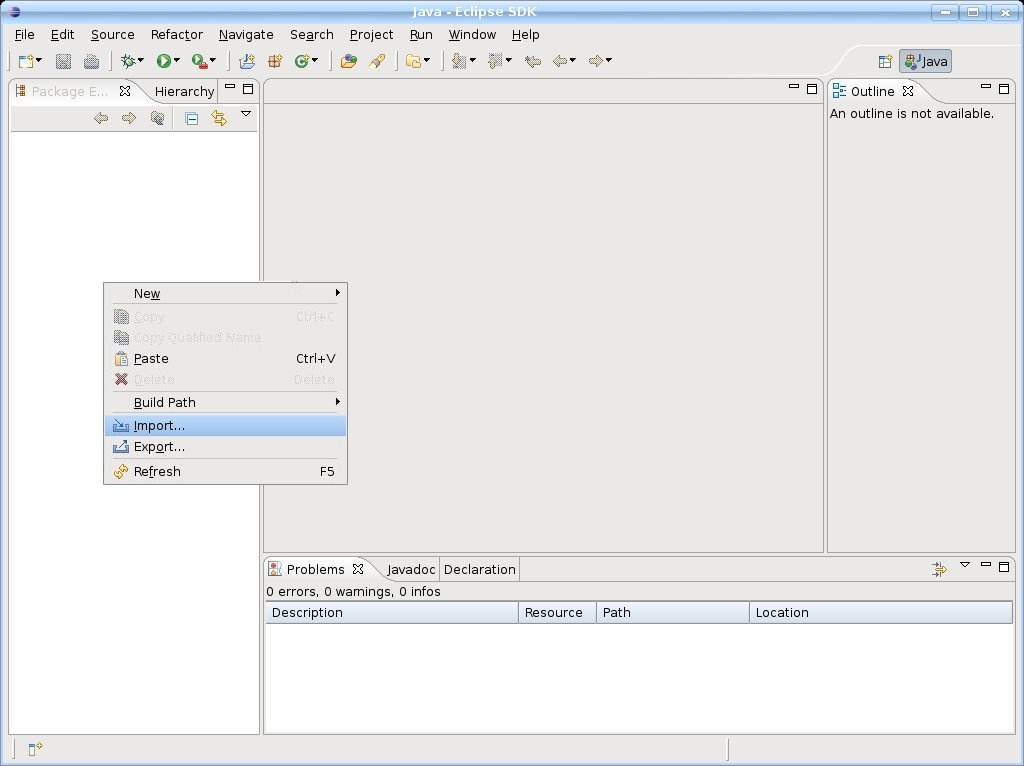
\includegraphics[width=0.6\linewidth]{img/eclipse-import}
\end{center}

\item Right click in the Package Explorer panel and select 'import' (or go in File/import)

\begin{center}
  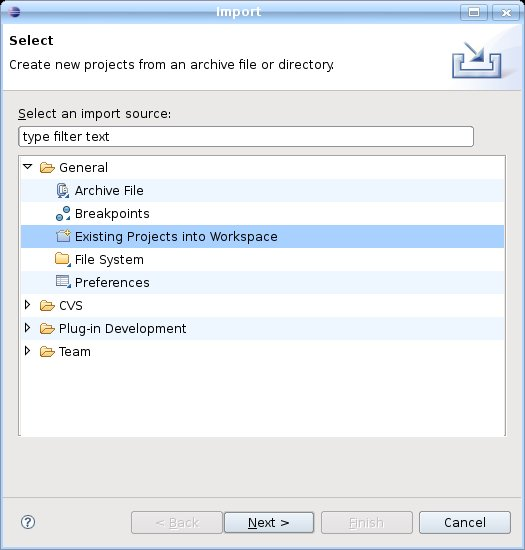
\includegraphics[width=0.6\linewidth]{img/select-import}
\end{center}

\item Select 'Existing Projects into Workspace' in the opened windows
\item Click 'Next'

\begin{center}
  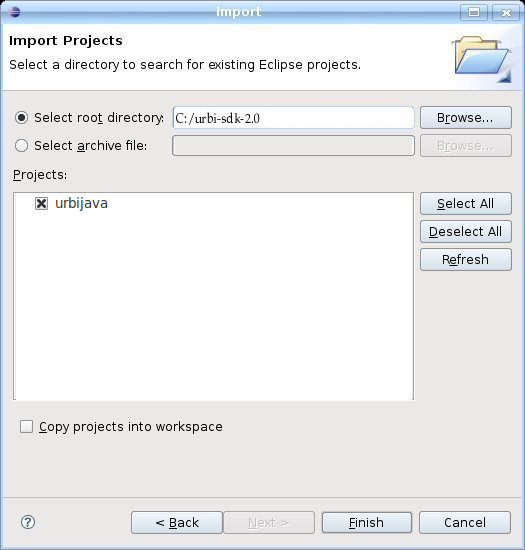
\includegraphics[width=0.6\linewidth]{img/select-proj}
\end{center}

\item Enter the path of the \urbi SDK on your computer
\item Eclipse should find the .project file we provide and display the 'urbijava' project
\item Select the 'urbijava' project and click 'Finish'

\begin{center}
  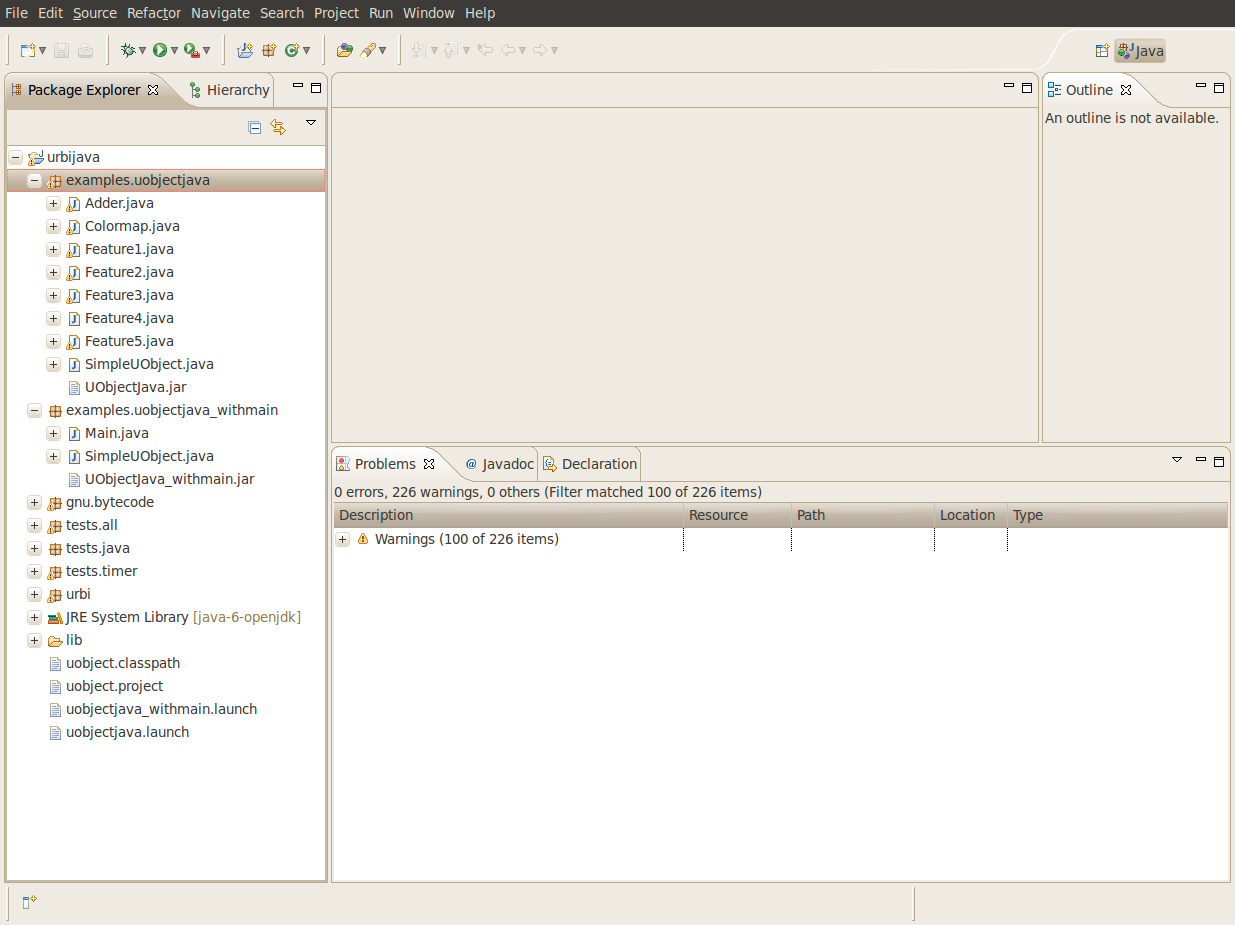
\includegraphics[width=0.6\linewidth]{img/project-uobject-open}
\end{center}

\end{itemize}

The Java project is loaded. You can see the jar containing the liburbi
(liburbijava.jar, storing the UObject Java API) which contains the urbi package, and
also see the sources of the example we provide. We put them in the packages
examples.  You can inspire yourself from these examples to make
your own UObjects.  Here, we will see how to compile and run them in eclipse

NB: If Eclipse complains about errors in the source code, it can be that
your compiler compliance level is two low. You have to set the compiler
compliance level to Java 5 at least (Windows/Preferences/Java/Compiler).

\begin{center}
  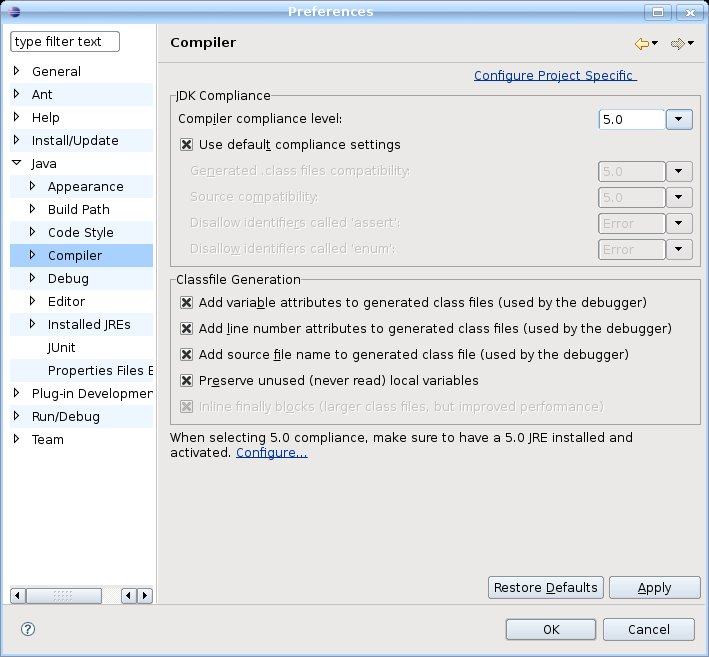
\includegraphics[width=0.6\linewidth]{img/compiler-compliance-level}
\end{center}


\section{Run the UObject Java examples}
\label{sec:uob:apijava:import}


We provide a sample uobjectjava.launch files that you can load in eclipse to
run the projects.

\begin{itemize}
\item Click on Run/Open Run Dialog (or 'Run...' or 'Run Configurations' in
  some versions of Eclipse)

\begin{center}
  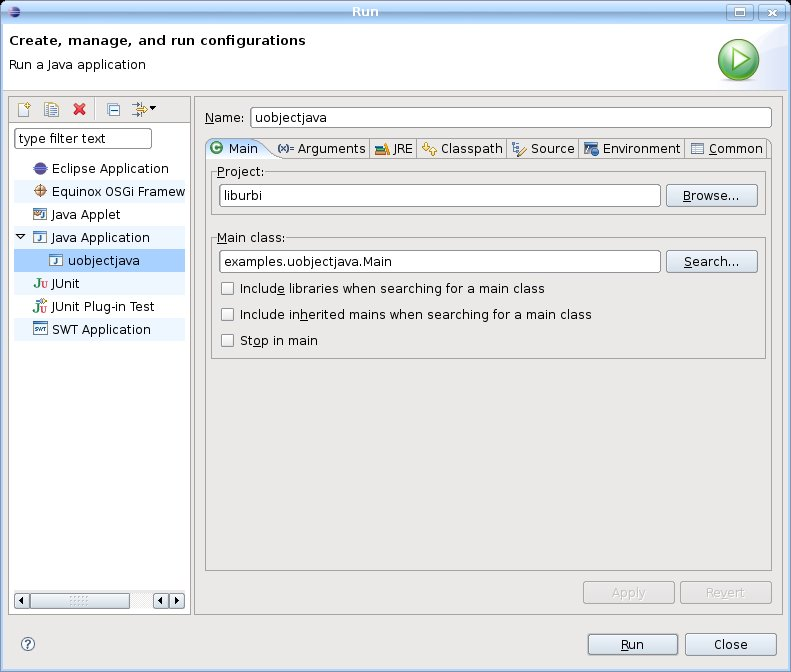
\includegraphics[width=0.6\linewidth]{img/run-uobjectjava}
\end{center}

\item The launch configurations should be recognized automatically. Choose 'uobjectjava'.

\item The project needs to load the urbijava native library. To this end, it will search the special
java.library.path path. If this path is not correctly set, the example will trigger an error.
You have to add to java.library.path the path to the \var{lib} folder in the \urbi SDK. You can do
this from the 'Run' menu, by selecting the 'Arguments' tab, and setting -Djava.library.path=\var{path to lib folder}
into the VM arguments. See:

\begin{center}
  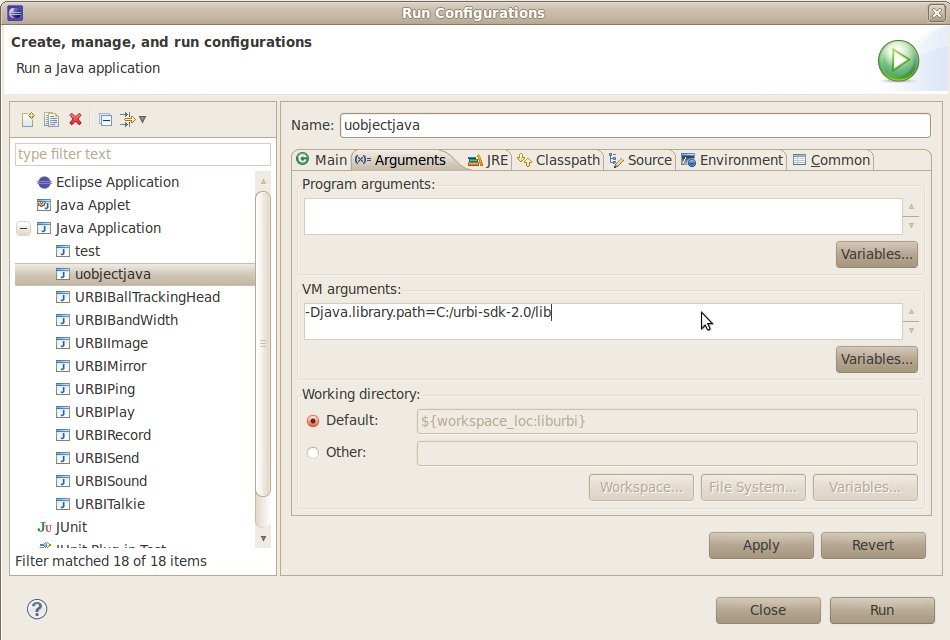
\includegraphics[width=0.6\linewidth]{img/set_javalibrarypath}
\end{center}

\item In order to run your remote UObject, you need also run an \urbi server. Your remote UObject
will connect to this \urbi server. By default \urbi servers listen on port 54000, and remote UObjects
try to connect to localhost on port 54000. If your urbi server is running on a different port or different
address, then you will need to give these port and address as argument to your program, in the 'Arguments'
tab (something like: -H address -P port). You can also write "--help" in this field, and then when you will
run the program it will display some help on the arguments available.

\item Click 'Apply'. Click 'Run'.

\end{itemize}

%%% Local Variables:
%%% mode: latex
%%% TeX-master: "../urbi-sdk"
%%% ispell-dictionary: "american"
%%% ispell-personal-dictionary: "../urbi.dict"
%%% fill-column: 76
%%% End:
